\documentclass[
    parskip=half, 
    twoside=false,
    twocolumn=true,
    fontsize=11pt,
]{scrarticle}
\usepackage{xcolor}
\definecolor{seeblau}{HTML}{00A9E0}
\definecolor{seegrau}{HTML}{9AA0A7}

\definecolor{seeblau1}{HTML}{CCEEF9}
\definecolor{seeblau2}{HTML}{A6E1F4}
\definecolor{seeblau3}{HTML}{59C7EB}
\definecolor{seeblau4}{HTML}{00A9E0}
\definecolor{seeblau5}{HTML}{008ECE}


\usepackage{graphicx}
\usepackage{amsmath}
\usepackage{subcaption}
\usepackage{wrapfig}
\usepackage[english]{babel}
\usepackage{blindtext}
\usepackage{microtype}
\usepackage{siunitx}
\usepackage[utf8]{inputenc}
\usepackage{csquotes}
\usepackage{nicefrac}
\usepackage[T1]{fontenc}
\usepackage{amsfonts}
\usepackage{amssymb}
\usepackage{tikz}

\usepackage{siunitx}

\usepackage{libertinus, libertinust1math}
\usepackage{roboto}

\setkomafont{disposition}{\normalfont\sffamily}


% not recommended with KOMA-script
% make table of contents sans-serif
% \usepackage{tocloft}
% \renewcommand\cftchappagefont{\normalfont}
% \renewcommand\cftchapfont{\normalfont}
% \renewcommand\cftchappresnum{\bfseries}
% \renewcommand\cftchapaftersnum{}
% \renewcommand{\cftchapfont}{\sffamily}
% \renewcommand{\cftsecfont}{\sffamily}
% \renewcommand{\cftsubsecfont}{\sffamily}
% \renewcommand{\cftchappagefont}{\sffamily}
% \renewcommand{\cftsecpagefont}{\sffamily}
% \renewcommand{\cftsubsecpagefont}{\sffamily}

% caption
\usepackage{caption}
\captionsetup{
	% font={sf},
	labelfont={sf, bf, color=seeblau},
	labelsep=quad,
	labelformat=simple,
}

% links
\usepackage{hyperref}
\hypersetup{
	colorlinks=true,
	linkcolor=seeblau,
	citecolor=seeblau,
	urlcolor=seeblau,
	% hidelinks=true
}

% bibliography
\usepackage[
	style=numeric-comp, % comp = compressed 4,5,6,7 -> 4-7
	sorting=none,		% Sort by appearance
	% autocite = superscript,
	% backref=true,
	hyperref=true,
	url=true,
	maxbibnames=100
]{biblatex}
\DefineBibliographyStrings{english}{%
    backrefpage  = {see p.}, % for single page number
    backrefpages = {see pp.} % for multiple page numbers
}

% remove issue
\AtEveryBibitem{%
  \clearfield{number}
}

\usepackage{float}
% \floatplacement{figure}{h}
% \floatplacement{table}{H}

% loosen float placement rules
\renewcommand{\topfraction}{0.8}
\renewcommand{\bottomfraction}{.8}
\renewcommand{\textfraction}{0.1}
\renewcommand{\floatpagefraction}{.9}
% make floats less likely to be placed on a separate page
\setcounter{totalnumber}{9}
\setcounter{topnumber}{9}
\setcounter{bottomnumber}{9}

% decrease space between floats and text
\setlength{\textfloatsep}{0.5cm}
\setlength{\floatsep}{0.5cm}


\usepackage{adjustbox}

\usepackage{datetime}
\newdateformat{dotdate}{
	\twodigit{\THEDAY}.\twodigit{\THEMONTH}.\THEYEAR
}
\newdateformat{monthyeardate}{%
  \monthname[\THEMONTH] \THEYEAR}


% header and footer
\usepackage[
  markcase=noupper
]{scrlayer-scrpage}% activates pagestyle scrheadings automatically
\clearpairofpagestyles
\setkomafont{pageheadfoot}{\normalfont\sffamily}
\setkomafont{pagenumber}{\normalfont\sffamily}
% \chead*{\color{seegrau} Draft \dotdate\today}
\ofoot*{\pagemark}
\ohead*{\rightmark}


\usepackage{ifthen}
\newcommand{\markieren}[4]{
    \ifthenelse{\equal{#1}{}}{}{\adjustbox{padding=3pt, bgcolor=seeblau1, margin=-1pt}{\strut{\sffamily\robotoMedium{#1}}}\\}
    \ifthenelse{\equal{#2}{}}{}{\adjustbox{padding=3pt, bgcolor=seeblau2, margin=-1pt}{\strut{\sffamily\robotoMedium{#2}}}\\}
	\ifthenelse{\equal{#3}{}}{}{\adjustbox{padding=3pt, bgcolor=seeblau3, margin=-1pt}{\strut{\sffamily\robotoMedium{#3}}}\\}
	\ifthenelse{\equal{#4}{}}{}{\adjustbox{padding=3pt, bgcolor=seeblau4, margin=-1pt}{\strut{\sffamily\robotoMedium{#4}}}}
}


\begin{document}

\title{title}
\subtitle{subtitle}
\author{Aurel Müller-Schoenau, Leon Oleschko}
\date{\dotdate\today}


% make a custom title page
\begin{titlepage}
    \sffamily
    \vspace*{3cm}
    {
        \fontsize{32}{32}
        \markieren{}{}{}{Rauschen}
    }
    \vspace{.25cm}\\
    {
        \Large
        Aurel Müller-Schoenau, Leon Oleschko\\
        Supervised by Richard Schlitz
        \vspace{.05cm}\\
        27. November 2024
        \vspace{.25cm}\\
        \normalsize
        Physikalisches Fortgeschrittenenpraktikum 2\\
        Universität Konstanz
    }
    \vfill
    {
        \normalfont\normalsize
        
    }
    \vfill
    \begin{flushright}
        Available at \url{www.github.com/leoole100/fp2}.
    \end{flushright}
\end{titlepage}

\section{Introduction}

\section{Setup}
The statistical uncertainty of the used voltmeter was measured to be $\sigma = \SI{0.001}{V}$ in the used range.

\subsection*{Oscilloscope RMS Measurement}


\section{Johnson-Nyquist Noise}
\begin{figure*}[h!]
    \centering
    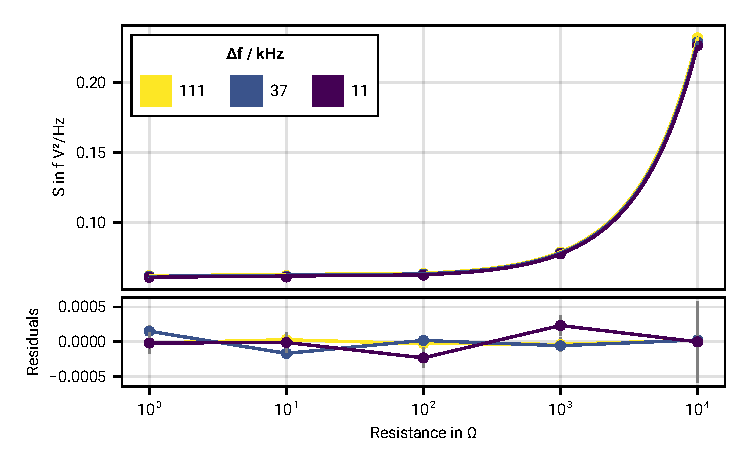
\includegraphics{figures/01 johnson noise.pdf}
    \caption{
        Measured noise density over different resistors for different bandwidths.
        Linear fit residuals are shown in the lower plot.
        Uncertainties are estimated using the Uncertainties of the voltage measurements.
        The uncertainties of the resistors and the amplifiers are not considered.
    }
    \label{fig:johnson noise}
\end{figure*}

\begin{equation}
    S = 4\; k_B T\; R + S_0
\end{equation} 
Therefore $k_B T$ and the amplifier noise $S_0$ can be measured from the fit in \autoref{fig:johnson noise}.
Assuming $T=\SI{295(3)}{K}$, the measured value for $k_B$ is $\SI{1.416(19)e-23}{J/K}$, which is off the literature value of $\SI{1.380e-23}{J/K}$.
The amplifier noise is measured to be $\SI{6.168(55)e-17}{V^2/Hz}$.

\subsubsection*{Temperature Measurement}
\begin{figure*}[h!]
    \centering
    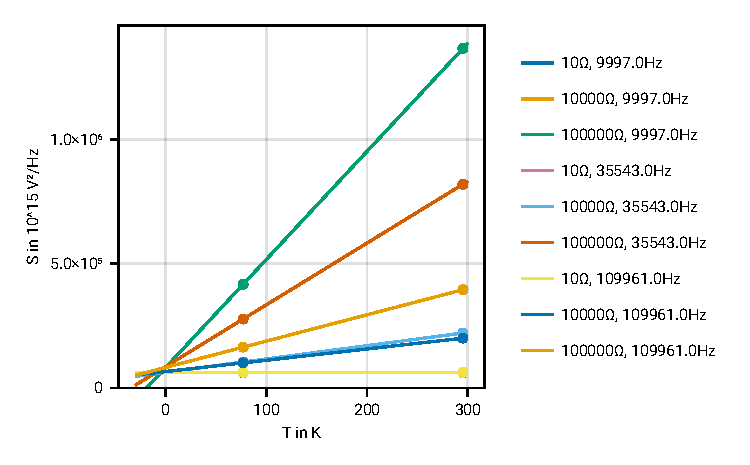
\includegraphics{figures/02 temperature.pdf}
    \caption{
        Measured noise density over temperature for different resistors and bandwidths.
    }
    \label{fig:johnson noise temperature}
\end{figure*}
\begin{figure}[h!]
    \centering
    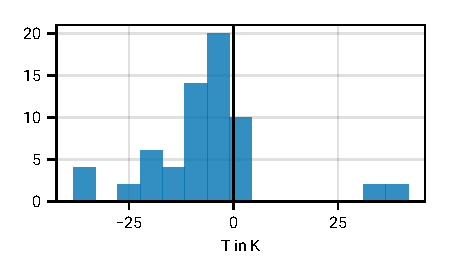
\includegraphics{figures/02 temperature distribution.pdf}
    \caption{
        Distribution of the measured temperature by looking at the crossings of the linear fits in \autoref{fig:johnson noise temperature}.
    }
    \label{fig:johnson noise temperature distribution}
\end{figure}
The measured zero temperature is \SI{-6.4(15)}{K}, the uncertainty is only including the spread.

\section{Shot Noise}
\begin{figure}[h!]
    \centering
    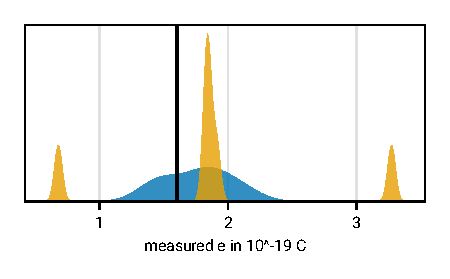
\includegraphics{figures/03 shot noise.pdf}
    \caption{
        Distribution of the measured value for $e$, by measuring the voltage over a resistor (blue) and using a transimpedance amplifier (yellow).
    }
    \label{fig:shot noise}
\end{figure}
The estimated values for $e$ using the two methods respectively are $\SI{1.76(25)e-19}{C}$ and $\SI{1.9(82)e-19}{C}$, which are both in agreement with the literature value of $\SI{1.602e-19}{C}$.
\textbf{Why is the second Uncertainty so high? See Histogram.}

\pagebreak
\section{Discussion}


\end{document}